\chapter{Inductances et transformateurs}
\section{Tensions appliquées et induites}
Si un circuit circulaire fermé est traversé par un flux variant, 
une f.e.m. induite se créera dans le même sens que le courant $i$ 
qu'elle génère : $e = -\dfrac{d\phi}{dt}$. Par la convention 
récepteur, la tension qui équilibre cette force doit avoir un 
sens opposé au courant. On a donc
\begin{equation}
\begin{array}{ll}
v &= Ri - e\\
 &= Ri + \dfrac{d\phi}{dt}
\end{array}
\label{eq:Maxou}
\end{equation}
On considérera que $e$ est définie dans le même sens que $v$ (on 
la voit comme une tension appliquée).

\section{Le transformateur idéal}
		\begin{wrapfigure}[9]{l}{2.5cm}
		\vspace{-5mm}
		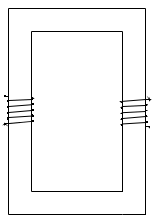
\includegraphics[scale=0.4]{ch3/image1.png}
		\captionof{figure}{ }
		\end{wrapfigure}
Soit l'illustration ci-contre avec $N_1$ et $N_2$ spires à gauche 
et à droite. Supposons que la résistivité du fer soit nulle : tout 
le flux va passer dans le fer et le flux perçu par les deux bobines 
sera identique. On définit alors le \textbf{flux totalisé} $\Psi$ 
comme le flux enserré par l'ensemble des $N$ spires d'un enroulement :
\begin{equation}
\Psi = N\phi
\end{equation}
où $\phi$ est le flux d'une spire. La loi de Maxwell (\autoref{eq:Maxou} 
où $R=0$) devient $v = \frac{d\Psi}{dt} = N\frac{d\phi}{dt}$. Comme le flux 
est le même dans les deux enroulements
\begin{equation}
\frac{\Psi_1}{\Psi_2} = \dfrac{N_1}{N_2},\qquad \frac{v_1}{v_2} = 
\frac{N_1}{N_2} = \mu.
\end{equation}
où $\mu$ est le rapport théorique des tensions. La loi des f.m.m 
donne
\begin{equation}
N_1i_1 + N_2i_2 = \underbrace{\oint_l \vec{H}.\vec{dl}}_{=0
\Leftrightarrow \mu_{Fe}=\infty}
\end{equation}
On sait que $\mu_0 \ll \mu_{Fe}$. Poussons le bouchon un peu plus 
loin : $\mu_{Fe} = \infty$. Imposer $v_1$ au montage donne un champ 
d'induction fini, mais un champ magnétique tendant vers 0 : dans un 
fer parfait, il faut une très petite force magnétomotrice ($\sum i$) 
pour faire circuler un flux. On a alors
\begin{equation}
N_1i_1 + N_2i_2 =0\quad\Leftrightarrow\quad \frac{i_1}{i_2} = -
\frac{N_2}{N_1} = -\frac{1}{\mu}
\end{equation}
Ceci décrit le transformateur idéal.

\newpage
\section{Inductances}
	\subsection{Inductances monophasées dans l'air}
		\subsubsection{Cas d'une seule spire}
				\begin{wrapfigure}[9]{r}{2.5cm}
		\vspace{-5mm}
		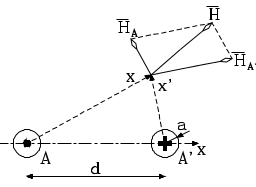
\includegraphics[scale=0.4]{ch3/image2.png}
		\captionof{figure}{ }
		\end{wrapfigure}
		Le flux passant à travers une spire est donné par $\phi = 
		LI$ où 		$L$ est l'inductance du circuit.\\
		\textsc{Exemple : calcul de $L$}. Si la spire est constituée 
		de deux conducteurs infini de rayon $a$, distant de $d$, 
		véhiculant un courant $i$, on peut calculer l'inductance de 
		ce circuit
		\begin{equation}
		\oint \vec{H}.\vec{dl} = \sum i\quad\Rightarrow\quad \left\{
		\begin{array}{ll}
		H_A &= \dfrac{i}{2\pi x}\\
		H_{A'} &= \dfrac{i}{2\pi(d-x)}		
		\end{array}\right.
		\end{equation}
		Comme $\int\vec{B}.d\vec{S} = \phi = \mu_0\int\vec{H}.d\vec{S}$ :
		\begin{equation}
		\phi = \frac{\mu_0}{2\pi}\int_{a}^{d-a}\left(\frac{1}{x}+
		\frac{1}{d-x}\right) i \text{ dx} = \frac{\mu_0}{\pi}\ln
		\frac{d-a}{a}i
		\end{equation}
		L'inductance \textbf{par unité de longueur} vaut alors (par 
		identification 	avec $\phi = Li$)
		\begin{equation}
		l = \frac{\mu_0}{\pi}\ln\frac{d-a}{a}\approx\frac{\mu_0}{
		\pi}\ln\frac{d
		}{a}
		\end{equation}
		
		\begin{center}
		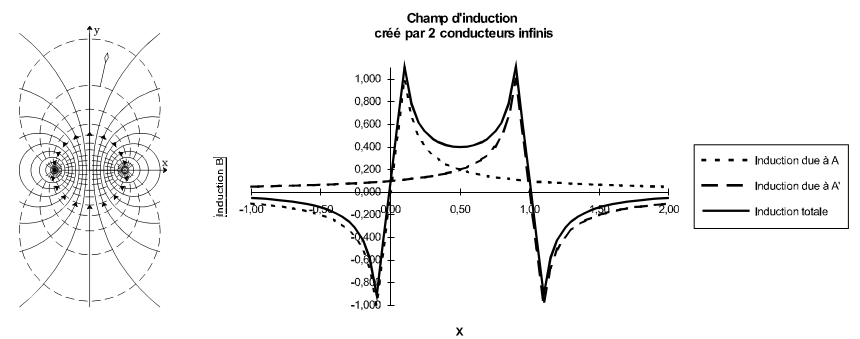
\includegraphics[scale=0.54]{ch3/image3.png}
		\captionof{figure}{ }
		\end{center}
		Les lignes de champ sont perpendiculaires au plan du conducteur. Les 
		cercles interrompus délimitent une même distance de la source ; il 
		s'agit d'équipotentielle magnétique. Sur une de ces lignes, à 
		n'importe quel point, la consommation en ampère-tour est la même 
		\begin{equation}
		\int\vec{H}.\vec{dl} = I = \text{ identique}
		\end{equation}
		Les lignes de champ se bouclent toujours, ou divergent à l'infini 
		(div $\vec{B}=0$). Sur le schéma de droite ci-dessus est répresenté 
		$B$ en fonction de la distance par rapports aux conducteurs $A$ et 
		$A'$, placés la où $B=0$. L' (champ) induction totale n'est que la 
		somme des inductions. On suppose également que le conducteur a un 
		certain rayon dans lequel on observe une croissance linéaire. Pour 
		retrouver $L$ à partir de ce graphique, il faut l'intégrer (aire sous 
		la courbe) et diviser par $I$.
		
		\subsubsection{Cas de plusieurs spires - Notions de flux 
		totalisé}
		La généralisation à $N$ spires est immédiate : $\Psi = 
		N\phi$ où $\phi$ est le flux d'une seule spire. Maxwell 
		se généralise de la même façon :
		\begin{equation}
		v = \frac{d\Psi}{dt} = N\frac{d\phi}{dt}\qquad\qquad\left(
		\begin{array}{ll}
		e_{spire} &= \frac{d\phi}{dt}\\
		e_{bobine} &= N\frac{d\phi}{dt} = \frac{d\Psi}{dt}
		\end{array}\right)
		\end{equation}
		Le milieu restant linéaire $\Psi = Li$. Grâce aux notions 
		du circuit magnétique et à la relation des Ampère-tours, on 
		peut écrire $Ni = \mathfrak{R}\phi$ où $\mathfrak{R}$ est la 
		\textbf{réluctance} du circuit d'induction. La valeur de l'
		inductance se calcule alors\footnote{On retrouve les mêmes formules, 
		mais avec $\Psi$.}
		\begin{equation}
		\Psi = Li = N\phi\quad \Leftrightarrow\quad L = \dfrac{\Psi}{i} = 
		N\dfrac{\phi}{i}
		\end{equation}
		$\text{Or, } Ni=\mathfrak{R}\phi$ :
		\begin{equation}
		\dfrac{\phi}{i} = \dfrac{N}{\mathfrak{R}}\qquad\longrightarrow\qquad 
		L = \frac{N^2}{\mathfrak{R}} 
		= N^2 \mathcal{P}
		\end{equation}
		où $\mathcal{P} = 1/\mathfrak{R}$ est la perméance du circuit. \\
		\danger Si les spires ne sont pas confondues la 
		relation $\Psi = N\phi$ n'est \textbf{plus} valable ! En effet, 
		le flux ne sera pas le même pour chaque spire : on appelle 
		flux de dispersion le flux non-commun. Bonne nouvelle : on est 
		encore dans une phase linéaire. En effet, nous sommes toujours 
		dans l'air qui est un milieu linéaire dans lequel on peut appliquer 
		le principe de superposition : flux $\propto I$. La relation  
		$\Psi = Li$ reste valable (et $L$ est constant tant que rien ne bouge).\\
		
		Petit rappel de vocabulaire : le flux "commun" sera dit de \textbf{magnétisation} 
		alors que le flux "non-commun" est dit de \textbf{dispersion}.		
		
		
	\subsection{Inductances monophasées à noyau magnétique}		
		\subsubsection{Flux et inductance}
		\begin{wrapfigure}[15]{l}{2.5cm}
		\vspace{-5mm}
		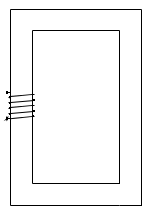
\includegraphics[scale=0.4]{ch3/image4.png}
		\captionof{figure}{Refermé sur lui-même pour avoir une inductance}
		\end{wrapfigure}
		Soit un circuit magnétique fermé de longueur $l$ et de section 
		constante $S$, constitué de $N$ spires. On suppose que le flux
		reste entièrement canalisé dans le fer\footnote{Très bonne 
		approximation} de sorte que $\Psi = N\phi$ reste valable\footnote{On 
		fait l'hypothèse que l'on a le même flux dans chaque spires, même si 
		celles-ci ne sont pas au même endroit.}.\\
		Le souci vient de l'imperfectibilité du fer : le relation entre 
		$\Psi$ et $i$ n'est plus linéaire : $\Psi = N\phi = BNS$ et 
		$i= H l/N$. Cette dernière relation est obtenue par la courbe 
		d'hystérèse magnétique qui n'est ni linéaire, ni univoque.\\
		
		Appliquons une tension sinusoïdale \textsc{alternative} $v = V_M\cos\omega t = V
		\sqrt{2}\cos\omega t$ à l'enroulement. Le flux résultant sera 
		sinusoïdal car $v = d\psi/dt$.	En première approximation, notre 
		tension vaut (toujours vrai):
		\begin{equation}
		v = Ri + \frac{d\Psi}{dt}
		\end{equation}
		Si la résistance est non-nulle, il faut résoudre un système à 
		deux inconnues\footnote{$\left\{\begin{array}{ll}
		v &= Ri + \frac{d\phi}{dt}\\
		Ni &\approx HL
		\end{array}\right.$} (dont une équation est donnée par le cycle d'
		hystérèse, Oh joie), la présence de $i$ compliquant l'ED. Par 
		contre, si $R=0$ :
		\begin{equation}
		\phi = \frac{\Psi}{N} = \frac{1}{N}\int_0^tv\text{ dt} + \text{ 
		cste}
		\end{equation}
		ce qui vaut\footnote{Q: Supposez qu'on ai une bobine comme ça et 
		que l'on met 12V. Si le courant est alternatif c'est un courant 
		alternatif. Représentez le ? Si on met du courant continu, on détruit la bobine 
		(ça fume, savoir expliqué).} $\phi = \frac{V_M}{N\omega}\cos\left(
		\omega t - \frac{\pi}{2}\right)$. Le phaseur $\underline{\phi}$ est 
		déphasé de $-\frac{\pi}{2}$ par rapport à $\underline{V}$. Grâce à la 
		relation $\phi = Li$, on peut voir ça intuitivement comme "$I$ est 
		en retard sur $V$ et on pourra modéliser ça par\dots une self !\\
		Comme $V_M = N\omega\phi_M$ :\footnote{??}
		\begin{equation}
		\phi_M = \dfrac{\sqrt{2}}{2\pi f N}V
		\end{equation}
		Si la tension appliquée est sinusoïdale, la tension et donc 
		l'induction le sera également, mais le courant absorbé par la 
		bobine ne l'est pas. On remarque que la valeur maximale de l'induction 
		ne dépend pas des propriété du matériau.
			
		\subsubsection{Courant absorbé}
		\begin{wrapfigure}[10]{r}{5.5cm}
%		\vspace{-10mm}
		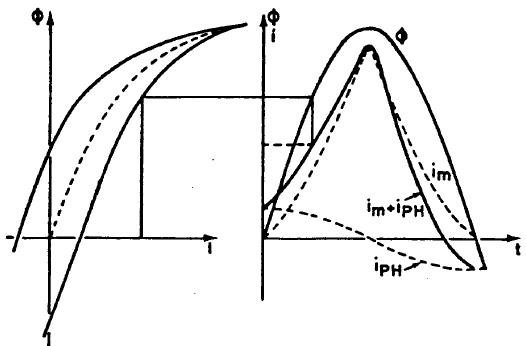
\includegraphics[scale=0.3]{ch3/image5.png}
		\captionof{figure}{Savoir expliquer ce graphique !}
		\end{wrapfigure}
		Sur le schéma ci-contre, $i_m$ 
		est le courant obtenu en ne considérant que la courbe d'aimantation 
		moyenne auquel il faut ajouter $i_{pH}$, le courant de pertes 
		hystérétiques pour donner le courant total $i$.
		
		
		\subsubsection{Pertes hystérétiques et par courants de Foucault}
		Si on place $i_{pH}$, le courant des pertes par hystérèse, sur un graphe
		 on va remarquer que sa courbe est en phase sur celle de la tension : 
		 on va pouvoir le modéliser par une résistance. Nous avons vu que 
		 $B^2\propto V^2$. On en déduit que la résistance sera à peu près 
		 constante et donc les pertes par hystérèse aussi.		\\
		 
		Compte-tenu de ceci, comment modéliser le courant ? On va simplement 
		mettre une inducance en parallèle avec une résistance pour retrouver 
		la somme de courant $i_p+i_m$ ! Le courant inductif sera plus grand 
		que le courant résistif car $R > L$ et comme on est en parralèle le 
		courant a plus de difficulté à circuler dans l'inductance que dans 
		la résistance. De plus, le fait d'être en parralèle implique que 
		le schéma équivalent sera, globalement, une inductance corrigée 
		par une résistance.
		
		\subsubsection{Schéma équivalent}
		Le courant absorbé par la bobine est composé d'un courant 
		magnétisant $I_m$ et un courant de pertes par hystérèse et par 
		Foucault $I_p$. On a vu que les pertes $\propto V^2$ et qu'elles 
		peuvent être représentées par une résistance $R_p$ de sort que 
		\begin{equation}
		\underline{V} = R_p\underline{I_p}
		\end{equation}
		\newpage
		\begin{wrapfigure}[10]{r}{5.5cm}
%		\vspace{-10mm}
		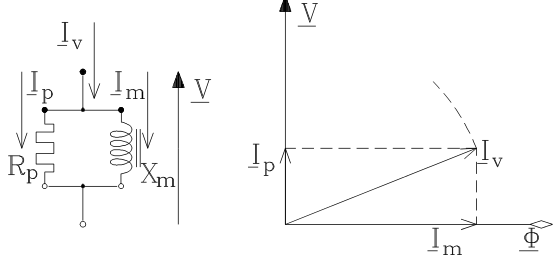
\includegraphics[scale=0.3]{ch3/image6.png}
		\captionof{figure}{ }
		\end{wrapfigure}
		Le courant magnétisant n'est pas sinusoïdal (car relation non-linéaire)
		mais on peut définir 
		un \textit{courant magnétisant sinusoïdal équivalent} déphasé de 
		$\pi/2$ sur la tension. L'idée est de remplacer $I_p$ par un courant 
		sinusoïdal de même valeur efficace
		\begin{equation}
		I_m= \sqrt{I_v^2-I_p^2}
		\end{equation}
		où $I_V = \sqrt{I_1^2+I_3^2+I_5^2+\dots}$. Dans cette expression, 
		$I_j$ est la valeur efficace de l'harmonique $j$ du courant. Il est 
		en effet habituel de définir un courant sinusoïdal équivalent de  
		même valeur efficace que le courant $i$ : $I_V = I$.\\
		Pour le fun, on peut définir une réactance de magnétisation $X_m : 
		\underline{V} = jX_m\underline{I}_m$, réactance qui dépend de l'état 
		de magnétisation du circuit. Ces constatations nous donnent le 
		schéma équivalent représenté ci-contre.
		
	\subsection{Inductance à circuit magnétique à entrefer}
		\begin{wrapfigure}[5]{l}{3.5cm}
		\vspace{-8mm}
		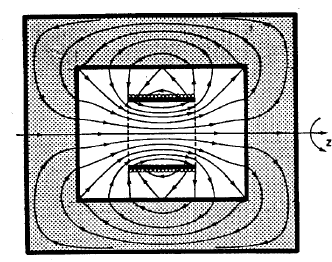
\includegraphics[scale=0.273]{ch3/image7.png}
		\captionof{figure}{ }
		\end{wrapfigure}
	La réluctance d'un tube de flux d'air d'1mm est équivalent à la 
	réluctance d'un tube de flux de 5000mm d'épaisseur dans le fer : l'
	inductance est essentiellement déterminée par l'entrefer : on peut le 
	voir comme un blindage magnétique.\\
	
	
	\subsection{Phénomènes transitoire de mise sous tension d'une bobine 
	de fer}
	Si on applique brusquement en $t=0$ la tension $v=V\sqrt{2}\cos(\omega 
	t+\xi_V)$ aux bornes d'une bobine idéale, le flux vaut\footnote{Par 
	intégration de $v = N\frac{d\phi}{dt}$.} (si l'on néglige le rémanent)
	\begin{equation}
	\begin{array}{ll}
	\phi &= \int_0^t \frac{V\sqrt{2}}{N}\cos(\omega t + \xi_V)\text{ dt}\\
	 &= \frac{V\sqrt{2}}{\omega N}\left[\cos(\omega t + \xi_V - \frac{\pi}{2})
	 -\cos(\xi_V-\frac{\pi}{2})\right]
	\end{array}	
	\end{equation}
	En tenant compte des résistances/pertes, le flux rejoint progressivement 
	sa valeur de régime sinusoïdal, de même pour le courant. Si l'enclenchement 
	se fait quand la tension est maximale ($\xi_V=0$), le flux est directement 
	en régime
	\begin{equation}
	\phi = \frac{V\sqrt{2}}{\omega N}\cos\left(\omega t - \frac{\pi}{2}\right)
	\end{equation}	
	Mais si on enclenche quand la tension est nulle ($\xi_v = -\frac{\pi}{2}$) :
	\begin{equation}
	\phi = \frac{V\sqrt{2}}{\omega N}[1-\cos\omega t]
	\end{equation}
	ce qui montre que le flux atteint deux fois la valeur de régime : le fer 
	peut se saturer (Voir explication labo avec l'aire sous la courbe).

\newpage
\section{Transformateurs monophasés}
	\subsection{Bobines à spires confondues, couplées dans l'air}
		\subsubsection{Introduction}
				\begin{wrapfigure}[5]{r}{3.5cm}
		\vspace{-27mm}
		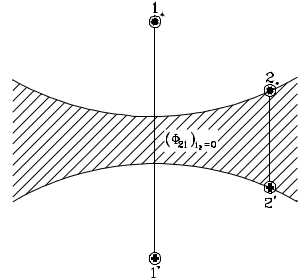
\includegraphics[scale=0.37]{ch3/image8.png}
		\captionof{figure}{Tout le flux créé par 1 n'arrive pas à 2}
		\end{wrapfigure}
		Soit deux bobines de $N_1$ et $N_2$ spires. Le point $\bullet$ marque 
		la borne d'entrée afin d'avoir une mutuelle positive. Comme le 
		système est linéaire (toujours dans l'air) la mutuelle $M$ est la même.
		\begin{equation}
		\begin{array}{ll}
		\Psi_1 &= L_1i_1 + Mi_2\\
		\Psi_2 &= Mi_1 + L_2i_2
		\end{array}
		\end{equation}
		En utilisant notre fameuse formule toujours vraie
		\begin{equation}
		\begin{array}{lll}
		v_1 &= R_1i_1 + \frac{d\Psi_1}{dt} &= R_1i_1 + L_1\frac{di_1}{dt}+M\frac{
		di_2}{dt}\\
		v_2 &= R_2i_2 + \frac{d\Psi_2}{dt} &= R_2i_2 + M\frac{di_1}{dt}+L_2\frac{
		di_2}{dt}
		\end{array}
		\end{equation}
		Ou encore
		\begin{equation}
		\begin{array}{ll}
		v_1 &= R_1i_1 + (L_1-M)\frac{di_1}{dt} + M\frac{d(i_1+i_2)}{dt}\\
		v_1 &= R_2i_2 + (L_2-M)\frac{di_2}{dt} + M\frac{d(i_1+i_2)}{dt}		
		\end{array}
		\end{equation}
		Cette équation peut directement être déduit du schéma suivant. 
		\begin{center}
				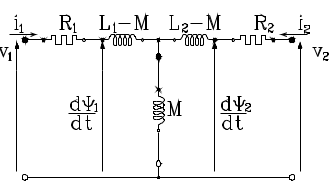
\includegraphics[scale=0.57]{ch3/image9.png}
		\captionof{figure}{ }
		\end{center}
		Hélas, on n'utilisera pas ce schéma car il peut conduire à des $L<0$. 
		Mathématiquement, tout est correct mais ce n'est physiquement pas 
		interprétable. Pour y remédier, on va introduire la notion de flux \textbf{commun} 
		et de \textbf{dispersion}.
		
		\subsubsection{Coefficients de couplage et de dispersion}
		$\triangleright$ Si $i_1$ (et $i_2=0$) parcoure la bobine 1, le flux se décompose en deux :
		\begin{enumerate}
		\item $\phi_{21}|_{i_2=0}$ est créée par 1 et coupée par 2
		\item $\phi_{d1}|_{i_2=0}$ est créé par 1, mais ne coupe par 2 : c'est le 
		\textit{flux de dispersion}
		\end{enumerate}
		Par définition, le coefficient de couplage $k_1$ est la fraction de flux 
		créer par une bobine qui atteint une autre :
		\begin{equation}
		k_1 \equiv \frac{\phi_{21}|_{i_2=0}}{\phi_1|_{i_2=0}}\leq 1
		\end{equation}
		où $k<1$ sauf si les bobines sont confondues ($k=1$).\\
		Reprenons nos équations fétiches (en considérant les spires confondues) :
		\begin{equation}
		\begin{array}{llll}
		\Psi_1|_{i_2=0} &= N_1\phi_1|_{i_2=0}& &= L_1i_1\\
		\Psi_2|_{i_2=0} &= N_2\phi_{21}|_{i_2=0}&= N_2k_1\phi_1|_{i_2=0} &= Mi_1		
		\end{array}
		\end{equation}
		En effectuant le rapport 
		\begin{equation}
		\left\{\begin{array}{ll}
		(\phi_1)_{i_2=0} &= \dfrac{L_1i_1}{N_1}\\
		N_2k_1(\phi_{21})_{i_2=0} &= Mi_1
		\end{array}\right.\qquad \Longrightarrow \qquad
		M = \frac{N_2}{N_1}k_1L_1\qquad \Leftrightarrow k_1 = \frac{N_1}{N_2}\frac{M}{L_1}
		\label{eq:3.23}
		\end{equation}
		$\triangleright$ Si $i_1=0$, un raisonnement similaire nous permet à partir de 
		\begin{equation}
		k_2 = \frac{(\phi_{12})_{i_1=0}}{(\phi_2)_{i_1=0}}
		\end{equation}
		d'obtenir 
		\begin{equation}
		M = \frac{N_1}{N_2}k_2L_2\qquad \text{ ou } k_1 = \frac{N_2}{N_1}\frac{M}{L_2}
		\end{equation}	
		Par définition, le couplage des deux bobines vaut
		\begin{equation}
		k = \sqrt{k_1k_2} = \frac{M}{\sqrt{L_1L_2}}
		\end{equation}
		Dans l'air, $k<0.5$. Par contre dans le fer $k \approx 0.998$.\\
		Le coefficient de Blondel est le rapport entre le flux de dispersion et le flux 
		total
		\begin{equation}
		\sigma_1 = \frac{(\phi_{dl})_{i_2=0}}{(\phi_1)_{i_2=0}} = 1-k_1\quad \rightarrow 
		\text{ facteur de dispersion de 1}
		\end{equation}
		
		\subsubsection{Couplage parfait}
		Comme on l'a dit : $k_1=k_2=1 \Rightarrow \phi_1=\phi_2$. On est dans le cas du 
		transformateur parfait (voir plus haut)
		
		\subsubsection{Schéma équivalent}
		Si $k_1>\frac{N_1}{N_2} \rightarrow M>L$ (via \autoref{eq:3.23}) et une 
		inductance négative serait 
		introduite : pas top, il va falloir procéder autrement. Remarquons que le 
		flux coupé par 1 est la somme des flux qu'il crée lui même et d'une fraction 
		du flux créé par 2 :
		\begin{equation}
		\Psi_1 = N_1(\phi_1)_{i_2=0} + N_1(\phi_{12})_{i_1=0}
		\end{equation}
		On peut décomposer $(\phi_1)_{i_2=0}$ en un flux de dispersion $(\phi_{dl})_{i_2=0}$ 
		et un flux 	coupé par l'enroulement 2 $(\phi_{21})_{i_2=0}$. Le flux commun est 
		le flux coupé par les deux 	enroulements :
		\begin{equation}
		\phi_C = (\phi_{21})_{i_2=0} + (\phi_{12})_{i_1=0}
		\end{equation}
		En considérant la décomposition proposée :
		\begin{equation}
		\Psi_1 = N_1((\phi_{dl})_{i_2=0}+(\phi_{21})_{i_2=0})+N_1(\phi_{12})_{i_1=0}
		\end{equation}
		On peut alors réécrire $\Psi_1$ :
		\begin{equation}
		\Psi_1 = N_1(\phi_{dl})_{i_2=0} + N_1\phi_C
		\end{equation}
		Reprenons la première équation de la section : $\Psi_1 = L_1i_1 + Mi_2$ et 
		décomposons le premier terme du second membre en:\footnote{$N_1\phi = \Psi$.}
		\begin{itemize}
		\item[$\bullet$] Flux de dispersion : $N_1(\phi_{dl})_{i_2=0} = (1-k_1)L_1i_i$.
		\item[$\bullet$] Flux commun : $N_1(\phi_{21})_{i_2=0} = k_1L_1i_1$.
		\end{itemize}
		Cette relation devient ainsi 
		\begin{equation}
		\Psi_1 = (1-k_1)L_1i_1 + (k_1L_1i_1 + Mi_2) = N_1(\phi_{dl})_{i_2=0} + N_1\phi_C
		\end{equation}
		Comme $k_1 = \frac{N_1}{N_2}\frac{M}{L_1} = \mu\frac{M}{L_1}$, on obtient
		\begin{equation}
		\Psi_1=	\displaystyle (L_1-\mu M)i_1 + \mu M\left(i_1+\dfrac{i_2}{\mu}\right)
		\end{equation}
		On peut faire le même raisonnement pour l'enroulement 2 (attention à la 
		définition de $k_2$ !)
		\begin{equation}
		\mu\Psi_2 = \mu^2\left(L_2-\frac{M}{\mu}\right)\frac{i_2}{\mu} + \mu M\left(
		i_1+\frac{i_2}{\mu}\right)
		\end{equation}
		Les deux dernières relations obtenues nous permettent de construire le 
		schéma équivalent suivant où $D$ est un opérateur dérivatif. Pour 
		construire ce schéma, il faut avant tout remarquer que le dernier terme 
		de ces deux équations est identique : il existe une "branche" commune.
		\begin{center}
		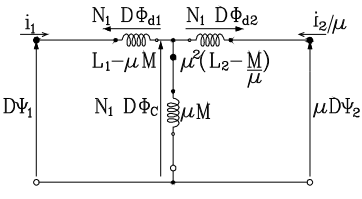
\includegraphics[scale=0.57]{ch3/image10.png}
		\captionof{figure}{ }
		\end{center}
		
		Le flux $\Psi_2$ et la tension $v_2$ secondaire sont \textbf{ramenés} (permet 
		l'interprétation physique) au primaire 
		par multiplication de $\mu$, alors que le courant doit être divisé par $
		\mu$. On ramène les impédances au primaire par multiplication de $\mu^2$.
		Si l'on tient compte des résistances des enroulement, on obtient le schéma 
		complet, où
		\begin{itemize}
		\item[$\bullet$] $L_{dl} = L_1-\mu M$ inductance de dispersion du primaire
		\item[$\bullet$] $L_{d2} = L_2-\frac{M}{\mu}$ inductance de dispersion du 
		secondaire
		\item[$\bullet$] $L_{d2}' = \mu^2L_{d2}$ inductance de dispersion ramenée au 
		primaire
		\item[$\bullet$] $\mu M$ inductance de magnétisation vue du primaire
		\end{itemize}
		Toutes ces grandeurs peuvent être ramenée au secondaire en multipliant les
		courants par $\mu$, les tensions par $1/\mu$ et les impédances par $1/\mu^2$ 
		comme le suggère le schéma ci-dessous.
		\begin{center}
		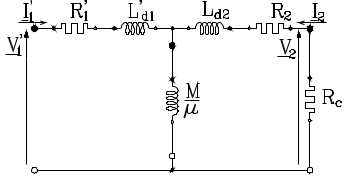
\includegraphics[scale=0.57]{ch3/image11.png}
		\captionof{figure}{ }
		\end{center}
		
		
		\subsubsection{Applications du schéma équivalent}
		Avec lui, on peut calculer le comportement statique et dynamique du 
		transformateur avec $R$ et $L$. Le rapport de transformation à vide, par 
		exemple, vaut\footnote{$v_1 = R_1i_1 + (L_1-\mu M)Di_1 + \mu MDi_2$.}
		\begin{equation}
		\left(\dfrac{v_1}{v_2}\right)_{i_2=0} = \mu\dfrac{R_1+L_1D}{\mu MD}
		\end{equation}
		La page 3.23 détaille la recherche de la courbe de réponse en fréquence 
		d'un transformateur (important). Ce rapport vaut $\mu/k$ si $R$ est 
		négligeable. Pour le cas parfait, on retrouve bien $\mu$. Plus il y 
		aura de la dispersion, plus ce rapport s'écartera de $\mu$.
		
	\subsection{Transformateurs à bobines couplées dans l'air}
		Le système étant linéaire, on peut écrire
		\begin{equation}
		\begin{array}{ll}
		\Psi_1 &= L_1i_1 + Mi_2\\
		\Psi_2 &= Mi_1 + L_2i_2
		\end{array}
		\end{equation}
		mais $\Psi_1=N_1\phi_1$ n'est plus valable car les flux coupés par chaque 
		spire d'un enroulement sont différent, on devra utiliser les coefficients 
		de couplages mesurés ou calculés.
		
%\newpage		
	\subsection{Transformateurs à noyau magnétique}
		\subsubsection{Transformateur sans dispersion}
		Par hypothèse, tout le flux passe dans le fer. les flux coupés par les deux 
		enroulements sont identiques :
		\begin{equation}
		\frac{\Psi_1}{\Psi_2} = \frac{N_1}{N_2}\qquad\text{ et }\qquad \frac{v_1}{
		v_2}=\frac{N_1}{N_2} = \mu
		\end{equation}
		Ce flux étant imposé par la tension, il est indépendants des courants :
		\begin{equation}
		V = \underbrace{Ri}_{\approx0} + \dfrac{d\Psi}{dt} \Rightarrow \Psi = f(V)
		\end{equation}				
		Le flux sera donc le même qu'à vide ($i_2 = 0$).
		Par la loi des f.m.m.
		\begin{equation}
		N_1i_1 + N_2i_2 = \oint_l \vec{H}.\vec{dl}
		\end{equation}
		où $l$ est une ligne d'induction dans le fer. Comme on l'a dit, le flux est le 
		même qu'à vide et donc $\vec{H}$ est aussi le même 
		qu'à vide : $\oint_l Hdl = N_1i_v$ où $i_v$ est le courant consommé 
		au primaire, à secondaire ouvert lorsque la tension appliquée $(v_m)$ est 
		la même qu'en charge : $v_1=v_2'$. On peut voir ce courant comme représentant à 
		la fois la magnétisation via la bobine et les pertes via la résistance.\\
		\begin{wrapfigure}[8]{l}{4cm}
		\vspace{-8mm}
		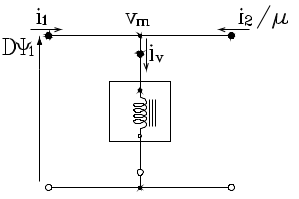
\includegraphics[scale=0.4]{ch3/imager1.png}
		\captionof{figure}{ }
		\end{wrapfigure}
		Comme nous avons la relation
		\begin{equation}
		i_1 + \frac{i_2}{\mu} = i_v
		\end{equation}
		il faut nécessairement introduire une bobine consommant $i_v$ sous la 
		tension $v_m$. 	\\
		Si l'on rajoute les résistances des impédances mais également une résistance 
		modélisant les pertes par hystérèse et courant de Foucault, on trouve le 
		schéma du transformateur non parfait standard.
	
		\begin{center}
		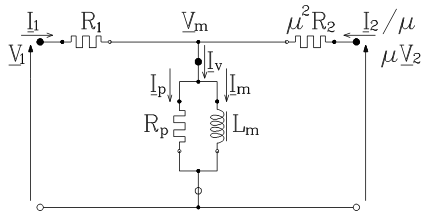
\includegraphics[scale=0.54]{ch3/imager2.png}
		\captionof{figure}{$L_m$ est l'inductance de dispersion}
		\label{fig:SchNnPrftStdr}
		\end{center}			
	
		\subsubsection{Transformateurs à spires concentrées}
		Dans ce cas on peut définir un flux commun $\phi_c$ et des flux de 
		dispersions $\phi_{d1},\phi_{d2}$ qui seront modélisés par des bobines. 
		Comme ceux-ci sont très faible, on 
		considère que le flux total est le flux commun. La \autoref{fig:SchNnPrftStdr}
		reste valable si l'on remplace le flux total par le flux commun, c'est-à-dire 
		si on pose $v_m = D\Psi_C=N_1D\phi_C$.
		Pour le premier enroulement
		\begin{equation}
		\begin{array}{ll}
		v_1 &= R_1i_1 + D\Psi_1\\
		&= R_1i_1 + D(\Psi_{d1}+\Psi_C)\\
		&= R_1i_1 + N_1D(\phi_{d1}+\phi_C)
		\end{array}
		\end{equation}
		Comme le flux de dispersion est dans l'air, un milieu linéaire $\phi = Li_1$. 
		Donc
		\begin{equation}
		v_1 = R_1i_1 + L_{d1}Di_1+N_1D\phi_C
		\end{equation}
		\begin{wrapfigure}[13]{l}{8cm}
%		\vspace{-8mm}
		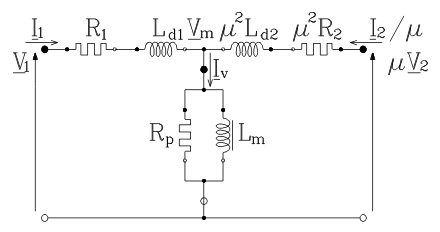
\includegraphics[scale=0.5]{ch3/imager3.png}
		\captionof{figure}{ }
		\end{wrapfigure}				
		Pour le second enroulement	
		\begin{equation}
		v_2 = R_2i_2 + L_{d2}Di_2+N_2D\phi_C
		\end{equation}	
		En ramenant le tout au primaire (comme fait précédemment)
		\begin{equation}
		\mu v_2 = \mu^2R_2\dfrac{i_2}{\mu}+\mu^2L_{d2}D\dfrac{i_2}{\mu}+N_1D\phi_C
		\end{equation}
		Et l'on trouve le schéma équivalent ci-contre.\\
		
		
		Petit exercice de réflexion? Supposons $R_1\ll \mu'R_2$. Cela signifierait 
		qu'une des résistances conduit à beaucoup plus de pertes : ce n'est pas 
		logique, l'ingénieur à mal fait son job.\\
		Notons que si on connaît les six impédances et $\mu$, on connaît tout!\\
		
		Les ordres de grandeurs sont important dans un tel schéma. Les voici 
		classées par ordre d'importance 
		\begin{enumerate}
		\item L'impédance la plus grande est dans la branche verticuale ($R_p \approx 
		3 L_m$)
		\item Les impédances de dispersions sont faibles mais plus grandes que 
		les résistances joules ($L_d \approx 10 R_1$).
		\item Si $\mu = 10$, la tension est 10 fois plus faible mais le courant 
		dix fois plus fort (conservation de la puissance). Comme les dissipations 
		doivent êtres les mêmes de chaque côté (sinon mauvais ingénieur) : $R_1 
		\approx \mu^2R_2, L_1\approx \mu^2L_2$.
		\end{enumerate}
		
	
		\subsubsection{Transformateurs réels}
		Dans le cas $\mathbb{R}$, les spires ne sont plus concentrée mais 
		supposer que $\phi_c = \phi_{Fe}$ reste valable de sorte que l'on 
		puisse utiliser nos schémas équivalents.	
	
		\subsubsection{Applications}
		La mesure de $R_p/L_m$ se fait à vide, car $R_1$ est négligeable devant 
		$R_p$. Pour mesurer le reste des impédances, on fait un court-circuit 
		au secondaire pour que $I_v\approx0$.
		
		
	\setcounter{subsection}{4}	
	\subsection{Pertes et rendement}
	La puissance au primaire est égale à la somme de la puissance dans la charge, 
	des pertes magnétiques et joules
	\begin{equation}
	P_1 = P_c + P_{pFe}  + P_{pCu}
	\end{equation}
	\begin{itemize}
	\item[$\bullet$] Les pertes magnétiques sont indépendantes de la charge et 
	se mesure à vide, car les pertes joules à vide sont très faibles.
	\item[$\bullet$] Les pertes joules se mesurent en court-circuit, car la tension 
	est faible et dès lors les pertes magnétiques sont souvent négligeables.
	\end{itemize}
	Le rendement est donné par\footnote{"Ne pas trop s'embêter avec les calculs"} :
	\begin{equation}
	\eta = \dfrac{P_c}{P_1} = \dfrac{P_c}{P_c+P_{pFe} + P_{pCu}}
	\end{equation}
	Après analyse, le rendement maximal est atteint pour une charge $P_c$ telle 
	que $P_{pFe} = P_{pCu}$.
	
	\begin{center}
	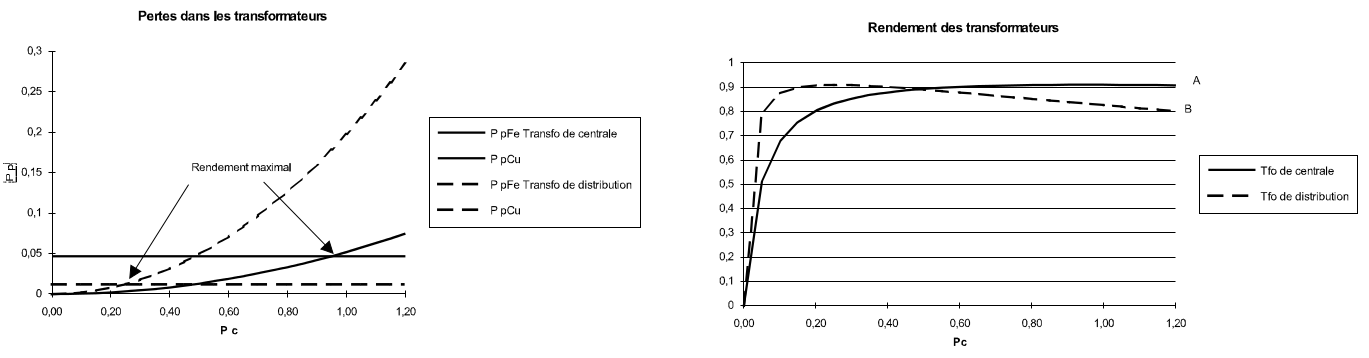
\includegraphics[scale=0.35]{ch3/imager4.png}
	\captionof{figure}{ }
	\end{center}
	Les pertes du transformateurs se divisent en deux
	\begin{enumerate}
	\item Les pertes augmentent avec le carré de la puissance, il s'agit de pertes
	quadratiques
	\item L'hystérèse et les courants de Foucault sont les pertes dans le fer même. 
	Celles-ci dépendent de la tension appliquée et non pas de la puissance.
	\end{enumerate}
\newpage	
\section{Transformateurs triphasés}
	\subsection{Constitution}
		\begin{wrapfigure}[17]{r}{8.5cm}
		\vspace{-8mm}
		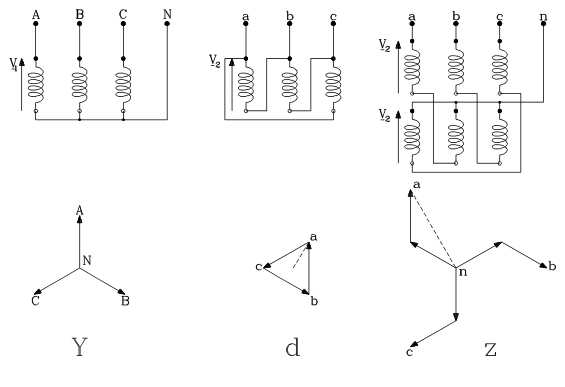
\includegraphics[scale=0.45]{ch3/imager5.png}
	\captionof{figure}{Transformateur primaire couplé en étoile, transformateur 
	secondaire en triangle et (droite) en zig-zag}
		\end{wrapfigure}				
	Il existe plusieurs façon de faire, la plus "classique" (dans ce cours) est de 
	considérer trois transformateurs monophasés indépendants dont les enroulements 
	sont connectés généralement en étoile (Y) ou en triangle ($\Delta$). Voyons, 
	ci-contre,	quelques dispositions particulières.
	La première chose à remarquer est qu'il y a chaque fois six bornes au primaire 
	et au secondaire (chaque fois deux accès). Dans le couplage en triangle, rien 
	n'empêche de permuter $a,b$ et $c$ : le déphasage ne sera juste plus de $30^\circ$ 
	mais de $120^\circ, -30^\circ,\dots$ Cela dépend donc de l'ordre dans lequel on 
	connecte les bobines. Toujours dans le triangle, la somme des tensions étant 
	forcément nulle, il n'y a pas de courant qui y circule (mais il en circule bien 
	dans chaque bobine). Le secondaire en zig-zag, c'est juste un truc d'hipster.
	
	\subsection{Fonctionnement en régime équilibre d'ordre direct}
		\subsubsection{Trois unités indépendantes}
		\begin{wrapfigure}[12]{r}{8.5cm}
		\vspace{-8mm}
		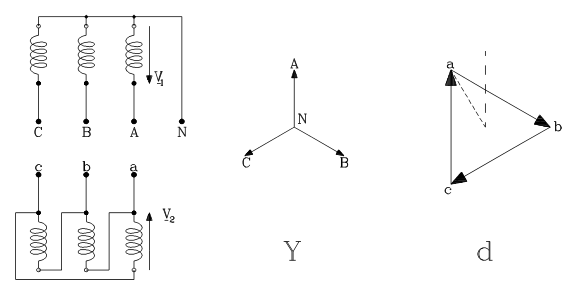
\includegraphics[scale=0.45]{ch3/imager6.png}
	\captionof{figure}{ }
		\end{wrapfigure}			
		Soit un transformateur $Yd$ auquel la tension primaire simple $\underline{V_1}$ 
		correspond la tension secondaire composée $\underline{V_2}$.\\

				Considérons la tension simple de la phase $A$ du primaire et $a$ du secondaire. 
		On obtient $V_a$ en divisant $\underline{V_2}$ par $\sqrt{3}$ ainsi qu'en 
		effectuant une rotation du phaseur de $30^\circ$. Le rapport de tension est 
		devenir $\mathbb{C}$ :
		\begin{equation}
		\mu \approx \dfrac{\underline{V_A}}{\underline{V_a}} = \dfrac{N_1}{N_2}\sqrt{3}
		\angle-30^\circ
		\end{equation}
	
		\subsubsection{Indice horaire $H$}
		Le déphasage primaire/secondaire dépend du couplage : on le caractérise par 
		l'indice horaire $H$, où $\underline{V_A}$ est placé à midi. Si $\underline{V_a}$ 
		est déphasé de $+30^\circ$, cela correspond à 11h. Un primaire en étoile, 
		un secondaire en triangle avec un déphasage de $30^\circ$ sera alors noté
		$Yd11$.\\
		
		En conclusion, le cas est identique au monophasé : il faut juste tenir compte 
		du facteur $\sqrt{3}$ et du déphasage.
	
	
	
	
	
	
	
	
	
	
	
	
	
	
	
	
	
	
	
	
	
	
